\chapter{Ground Data and Geomagnetic Indices}

	\section{\texttt{groundmag}: Tools for processing and reading ground magnetometer data}
	
	\section{\texttt{SuperDARN}: Simple SuperDARN fitacf reading code}

		\href{https://github.com/mattkjames7/SuperDARN}{https://github.com/mattkjames7/SuperDARN}

		The \texttt{SuperDARN} module is for reading and plotting SuperDARN fitacf files. It is a fairly simple tool, but use with caution because there may be some errors...

		\subsection{Installation}

			This package is not in the PyPI, so manual installation is necessary:
			\begin{minted}{bash}
#clone the repo
git clone https://github.com/mattkjames7/SuperDARN
cd SuperDARN

#build a Python package
python3 setup.py bdist_wheel

#install it (replace 0.1.0 with whatever version is built)
pip3 install dist/SuperDARN-0.1.0-py3-none-any.whl --user
			\end{minted}
			
			Once installed, the directory used to create the Python wheel file can be deleted. It can be uninstalled using \texttt{pip3 uninstall SuperDARN}.

			Before running for the first time, a couple of environment variables need to be set up to tell the module where to look for fitacf files and to say where it is able to store some files:
			\begin{minted}{bash}
#path to where FITACF files are stored 
#(this one is specific to SPECTRE)
export FITACF_PATH=/data/sol-ionosphere/fitacf
	
#path to where this module can create some files
#(this should be a path where you have write access)
export SUPERDARN_PATH=/some/other/path/SuperDARN
			\end{minted}

			This module will not currently run on Windows (as far as I am aware) because it requires the compilation of some C++ code which is not yet cross-platform.

		\subsubsection{Usage}
		
			In ipython, the first time this module is imported, it should attempt to download some files from the \href{https://github.com/SuperDARN/rst}{Radar Software Toolkit (RST)} which help in calculating the coordinates of the fields of view of each radar. These files are created in the path defined be the \texttt{\$SUPERDARN\_PATH} variable.

			\subsubsection{Reading Data}
				There are a few functions within \texttt{SuperDARN.Data} which provide objects containing data:

				\begin{minted}{python}
import SuperDARN as sd
			
#get the data from a single cell (Radar,Date,ut,Beam,Gate)
cdata = sd.Data.GetCellData('han',20020321,[22.0,24.0],9,25)
			
#or a whole beam of data (Radar,Date,ut,Beam)
bdata = sd.Data.GetBeamData('han',[20020321,20020322],[22.0,24.0],7)
			
#data for the whole field of view (Radar,Date,ut)
#in this case, the output is a dict where each key is a beam number
#pointing to a recarray for each beam as produced by GetBeamData
rdata = sd.Data.GetRadarData('han',[20020321,20020322],[22.0,23.0])
				\end{minted}
			
				In the above examples \texttt{bdata} and \texttt{cdata} are \texttt{numpy.recarray} objects, \texttt{rdata} is a \texttt{dict} object containing a \texttt{numpy.recarray} for each beam.
			
				The fitacf data are stored in memory once loaded so that they don't need to be re-read every time the data are requested. To check how much memory is in use and to clear it:
			
				\begin{minted}{python}
#check memory usage in MB
sd.Data.MemUsage()
		
#clear memory
sd.Data.ClearData()
				\end{minted}
			
			\subsubsection{Plotting Data}
			
				There are a bunch of very simple plotting functions, e.g.:
			
				\begin{minted}{python}
import matplotlib.pyplot as plt
			
#create a figure
plt.figure(figsize=(8,11))
			
#plot the power along a beam
ax0 = sd.Plot.RTIBeam('han',[20020321,20020322],[23.0,1.0],9,[20,35],
					Param='P_l',ShowScatter=True,fig=plt,
					maps=[2,3,0,0],scale=[1.0,100.0],zlog=True,
					cmap='gnuplot')
			
#the velocity
ax1 = sd.Plot.RTIBeam('han',[20020321,20020322],[23.0,1.0],9,[20,35],Param='V',
					fig=plt,maps=[2,3,1,0])
			
#velocity along a range of latitudes at a ~constant longitude of 105
ax2 = sd.Plot.RTILat('han',[20020321,20020322],[23.0,1.0],105.0,Param='V',
					fig=plt,maps=[2,3,0,1])
		
#velocity along a range of longitudes at a ~constant latitude of ~70
ax3 = sd.Plot.RTILon('han',[20020321,20020322],[23.0,1.0],70.0,Param='V',
					fig=plt,maps=[2,3,1,1])
			
#some specific cells
beams = [1,5,7,2,8,4,9]
gates = [20,26,33,22,25,21,29]
ax4 = sd.Plot.RTI('han',[20020321,20020322],[23.0,1.0],beams,gates,
					Param='V',fig=plt,maps=[2,3,0,2])
			
#totally different FOV plot
ax5 = sd.Plot.FOVData('han',20020321,23.5,Param='V',fig=plt,maps=[2,3,1,2])
			
			
plt.tight_layout()
				\end{minted}
			
				which should produce figure \ref{FigSDExample}.
			
				\begin{figure}
					\centering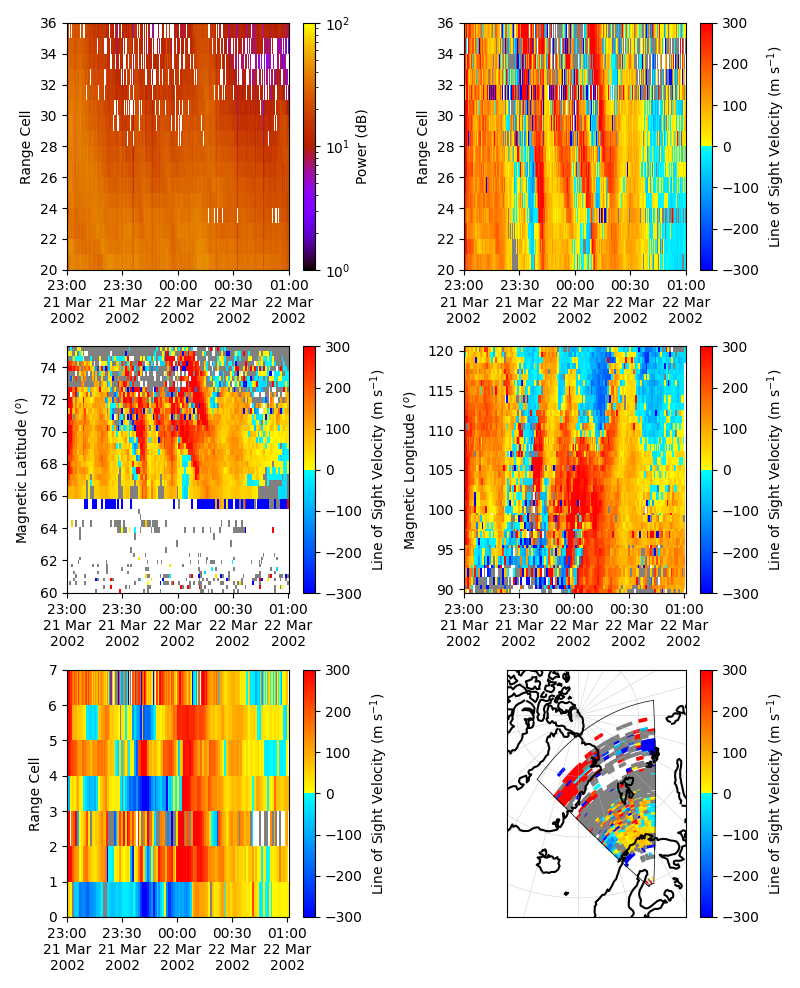
\includegraphics[width=0.8\textwidth]{figures/ch05_sdexample.png}
					\caption{Top left: range time intensity (RTI) plot of backscatter power. Top right: RTI plot of line of sight velocity. Mid left: velocity along a line of cells in magnetic longitude. Mid right: velocity along a range of longitudes. Bottom left: velocity of specific range cells. Bottom right: velocity within the field of view plot. \label{FigSDExample} }
				\end{figure}

			\subsubsection{Fields of View}
			
				These may be wrong. Use with great caution.
			
				The fields of view of each radar are stored as instances of the \texttt{SuperDARN.FOV.FOVObj} objects in memory and can be accessed using \texttt{GetFOV}, e.g.:
			
				\begin{minted}{python}
#get the object from memory
Date = 20020321
fov = sd.FOV.GetFOV('pyk',Date)
			
#use it to retrieve the FOV in mag coordinates
mlon,mlat = fov.GetFOV(Mag=True,Date=Date)
			
#plot it
ax = fov.PlotPolar(Background=[0.0,0.2,1.0],Continents=[0.0,1.0,0.2],
				color='magenta',ShowBeams=False,ShowCells=False,
				linewidth=2.0,Mag=True,Lon=True)
			
#add some cells
beams = [1,5,7,2,8,4,9]
gates = [20,26,33,22,25,21,29]
fov.PlotPolarCells(beams,gates,color='red',fig=ax,Mag=True,linewidth=2.0,Lon=True)
				\end{minted}
			
				The above code should look like figure \ref{FigSDFOV}:
			
				\begin{figure}
					\centering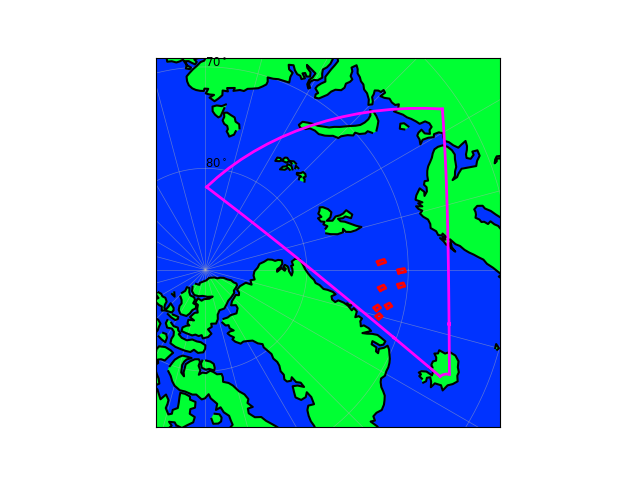
\includegraphics[width=0.5\textwidth]{figures/ch05_sdfov.png}
					\caption{SuperDARN field of view plot with specific cells highlighted.\label{FigSDFOV}}
					
				\end{figure}
			


	\section{\texttt{kpindex}: Download the latext Kp indices}

	Very simple package for obtaining the planetary Kp index data (see 
	\url{https://www.gfz-potsdam.de/en/kp-index/} for more information)
	
	\subsection{Installation}
	
	This package depends on the following:
	
	\begin{itemize}
	  \item numpy
	  \item RecarrayTools
	  \item PyFileIO
	\end{itemize}
	
	which are all available on PyPI.
	
	Installation is simple and can be done in one of four ways:
	
	\subsubsection{Method 1}
	
	This method simply uses the Python \texttt{pip3} command to download this 
	module and its dependencies:
	
	\begin{minted}{bash}
	pip3 install kpindex --user
	\end{minted}
	
	\subsubsection{Method 2}
	
	This method uses the Python wheel on the "releases" page of this 
	repository. Download the wheel, then install using \texttt{pip3}:
	
	\begin{minted}{bash}
	pip3 install kpindex-0.0.1-py3-none-any.whl --user
	\end{minted}
	
	\subsubsection{Method 3}
	
	Don't trust my prepackaged stuff? OK, clone this repository and build
	your own:
	
	\begin{minted}{bash}
	git clone https://github.com/mattkjames7/kpindex.git
	cd kpindex
	python3 setup.py bdist_wheel
	pip3 install dist/kpindex-0.0.1-py3-none-any.whl --user
	\end{minted}
	
	\subsubsection{Method 4}
	
	So you don't like wheels? Fine. Clone the repository and just move the
	"kpindex" folder to your \texttt{\$PYTHONPATH}.
	
	\subsection{Post-Install}
	
	In order for the module to be able to download the Kp index data from
	the FTP site, you will need to point it in the direction of a directory
	where you have read and write access using the \texttt{\$KPDATA\_PATH}
	environment variable. This can be done either by running the following
	in the terminal before starting Python, or inserting it into your 
	\texttt{\~{}/.bashrc} file:
	
	\begin{minted}{bash}
	export KPDATA_PATH=/path/to/the/data
	\end{minted}
	
	\subsection{Usage}
	
	Using this module is very simple: the first time you run it you will 
	need to update the database (also when you think the database is out of 
	date) e.g.
	
	\begin{minted}{python}
	import kpindex
	kpindex.UpdateLocalData()
	\end{minted}
	
	It may take a couple of minutes to download the data and convert it, 
	then you are ready to read the data:
	
	\begin{minted}{python}
	data = kpindex.GetKp(Date)
	\end{minted}
	
	where \texttt{Date} could be \texttt{None}, in which case ALL of the Kp indices ever
	will be returned; \texttt{Date} could be a single date in the format yyyymmdd,
	in which case only Kp indices from that date will be returned; finally,
	it could be a two-element array/list/tuple containing two dates, in this
	case, it will return all the indices from the start to the end date.
	
	Enjoy!
	

	\section{\texttt{pyomnidata}: Download the latext OMNI and solar flux data}


	Python tool for downloading, converting, and reading OMNI solar wind data.
	
	If you make use of the OMNI data please acknowledge and cite as specified here: \url{https://omniweb.gsfc.nasa.gov/html/citing.html}
	
	\subsection{Installation}
	
	Simply install using \texttt{pip3}:
	
	\begin{minted}{bash}
	pip3 install pyomnidata --user
	\end{minted}
	
	Alternatively install from this repository:
	
	\begin{minted}{bash}
	git clone https://github.com/mattkjames7/pyomnidata
	cd pyomnidata
	
	#EITHER build a wheel and install with pip (better)
	python3 setup.py bdist_wheel
	pip3 install dist/pyomnidata-1.0.0-py3-none-any.whl --user
	
	#OR directly using setup py (should work, not tested though)
	python3 setup.py install --user
	\end{minted}
	
	For this to work properly - you will need to set up the \texttt{\$OMNIDATA\_PATH} environment variable to point to a folder where you want to store the data. Do this by adding something along the lines of the following to the bottom of your \texttt{\~{}/.bashrc} file:
	
	\begin{minted}{bash}
	export OMNIDATA_PATH=/path/to/omni/data
	\end{minted}
	
	\subsection{Usage}
	
	\subsubsection{Downloading Data}
	
	Download OMNI data like this:
	
	\begin{minted}{python}
	import pyomnidata
	
	#download all available data
	pyomnidata.UpdateLocalData()
	\end{minted}
	
	Download F10.7 index (solar flux at 10.7 cm):
	
	\begin{minted}{python}
	pyomnidata.UpdateSolarFlux(EndDate=2021024)
	\end{minted}
	
	where \texttt{EndDate} is the last date for which you want to request solar flux data. This should be set to a date at least a few days prior to the current date. If you request a date that currently has no available data, the download will fail.
	
	\subsubsection{Read Data}
	
	Get the OMNI parameters like so:
	
	\begin{minted}{python}
	####OMNI parameters####
	#Year can either be a single year:
	Year = 2001
	#or it can be a range:
	Year = [2001,2004]
	
	#5 minute resolution data
	data = pyomnidata.GetOMNI(Year,Res=5)
	
	#1 minute data
	data = pyomnidata.GetOMNI(Year,Res=1)
	
	####solar flux###
	#all of the data
	data = pyomnidata.GetSolarFlux()
	
	#a single date
	data = pyomnidata.GetSolarFlux(Date=20050101)
	
	#a range of dates
	data = pyomnidata.GetSolarFlux(Date=[20020101,20020103])
	\end{minted}
	
	The returned \texttt{data} object is a \texttt{numpy.recarray} object which contains all of the OMNI data requested. To see what fields are stored use \texttt{print(data.dtype.names)}. The units are as presented here: \url{https://omniweb.gsfc.nasa.gov/html/omni_min_data.html#4b}
	
	\subsubsection{Plot Data}
	
	Use the \texttt{PlotOMNI} function, e.g.:
	
	\begin{minted}{python}
	import matplotlib.pyplot as plt
	
	#create a figure
	plt.figure(figsize=(11,6))
	
	#plot some stuff in one panel
	ax0 = pyomnidata.PlotOMNI(['SymH','SymD'],[20010101,20010120],fig=plt,maps=[2,1,0,0])
	
	#and a second panel
	ax1 = pyomnidata.PlotOMNI(['FlowSpeed'],[20010101,20010120],fig=plt,maps=[2,1,1,0])
	
	#fit things a bit nicer
	plt.tight_layout()
	\end{minted}
	
	Which should produce something like the following:
	
	\begin{figure}[H]
	  \centering
	  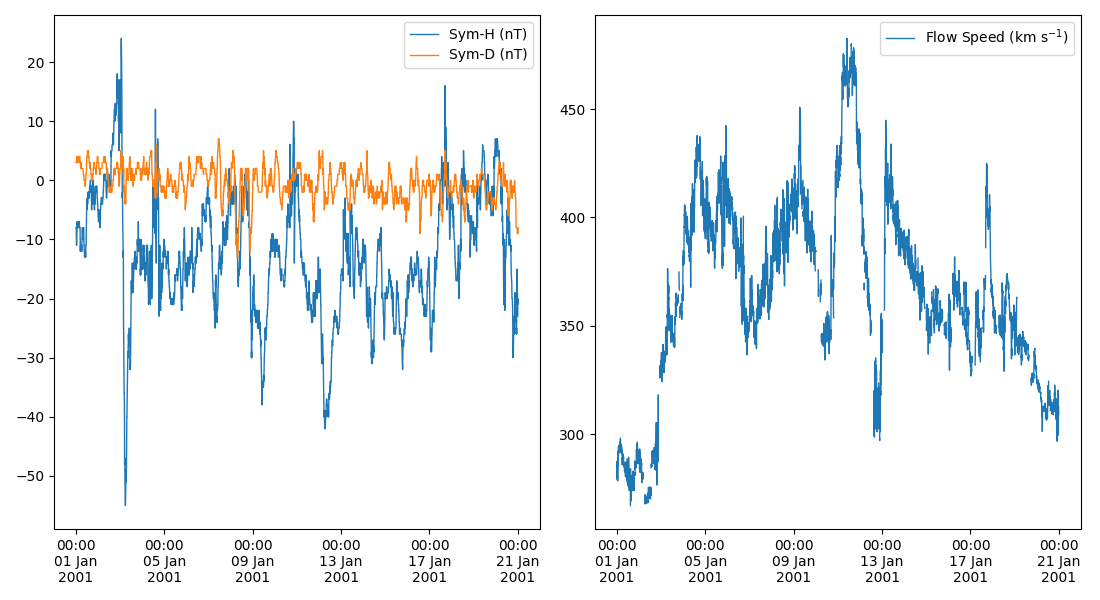
\includegraphics[width=\textwidth]{figures/ch5_omniexample.png}
	  \caption{Example plot using \texttt{pyomnidata}.}
	\end{figure}
	

	


	\section{\texttt{smindex}: Read the SuperMAG indices}


	A tiny module for reading SuperMAG indices and substorm lists.

	For the SuperMAG data visit \url{https://supermag.jhuapl.edu/indices}
	
	If using any of these data products, please remember to cite the relevant SuperMAG papers and acknowledge SuperMAG (see here: \url{https://supermag.jhuapl.edu/info/?page=rulesoftheroad})
	
	\subsection{Installation}
	
	Install this module using \texttt{pip3}:
	
	\begin{minted}{bash}
	pip3 install smindex --user
	\end{minted}
	
	Or by cloning and building this repository:
	
	\begin{minted}{bash}
	git clone https://github.com/mattkjames7/smindex
	cd smindex
	python3 setup.py bdist_wheel
	pip3 install dist/smindex-1.0.0-py3-none-any.whl --user
	\end{minted}
	
	Then set up an environment variable which points to where you want to store the data in your \texttt{\~{}/.bashrc} file:
	
	\begin{minted}{bash}
	export SMINDEX_PATH=/path/to/smindex/data/
	\end{minted}
	
	\subsection{Downloading Indices}
	
	For best results, visit the indices page on the SuperMAG website and select the following indices to download:
	
	SME U/L, SME, SME MLT, SME MLAT, SME LT, SMU LT, SML LT, SMR, SMR LT
	
	(follow this link: \url{https://supermag.jhuapl.edu/indices/?layers=SMR.LT,SMR,SMER.L,SMER.U,SMER.E,SME.MLAT,SME.MLT,SME.E,SME.UL&fidelity=low&start=2001-01-30T00%3A00%3A00.000Z&step=14400&tab=download})
	
	The data format should be ASCII and ideally download full-year files.
	
	These data files should then be placed in the directory \texttt{\$SMINDEX_PATH/download} where they can be processed.
	
	They can be converted to a binary format which is quick to read:
	
	\begin{minted}{python}
	import smindex
	smindex.ConvertData()
	\end{minted}
	
	\subsection{Read Indices}
	
	Use the \texttt{smindex.GetIndices} function to read the converted index files:
	
	\begin{minted}{python}
	#Read a single year file
	data = smindex.GetData(2005)
	
	#or a range of years
	data = smindex.GetData([2005,2008])
	\end{minted}
	
	\subsection{Downloading Substorm Lists}
	
	Substorm lists (by Frey et al., 2004 and 2006; Liou 2010; Newell and Gjerloev, 2011; Forsyth et al., 2015; Ohtani and Gjerloev, 2020) can be downloaded from the following page: \url{https://supermag.jhuapl.edu/substorms/?tab=download}
	
	The ASCII file format is readable by this module. The files should be placed in \texttt{\$SMINDEX_PATH/substorms}.
	
	Once you have all of the data files, they can be combined using the following function:
	
	\begin{minted}{python}
	smindex.UpdateSubstorms()
	\end{minted}
	
	\subsection{Reading Substorms}
	
	The best way to read the substorm lists is to use the \texttt{GetSubstorms} function:
	
	\begin{minted}{python}
	#get everything:
	ss = smindex.GetSubstorms()
	
	#get a single date (25th January 2005 in this case)
	ss = smindex.GetSubstorms(Date=20050125)
	
	#get a range of dates
	ss = smindex.GetSubstorms(Date=[20050101,20050125])
	\end{minted}
	


